\chapter{Understanding the problem}
\label{Introduzione}
\thispagestyle{empty}

\noindent Due to the huge impact of their consequences, the pursuit of forecasting earthquakes is one of the most important problems in Earth science. Studies that have been made so far focus on three key points: when, where and how large the event will be.

\section{Previous studies}
But how are these prediction achieved? Los Alamos National Laboratory has conducted a study on huge sets of laboratory experimental seismic data, showing the importance of the so called "slow earthquakes", which are still less understood. In their work \cite{sloweq}, the researchers try to spark some light on the mechanics of slow-slip phenomena and their relationship with regular earthquakes, to which they seem to be precursors, through a complete systematic experimental study.

\bigbreak

A second study, based on the results of laboratory experiments, takes advantages of Machine Learning techniques to predict the time to the next "labquake" by listening to the acoustic signal collected by specific laboratory sensors \cite{mleq}. By using ML, even small seismic precursor magnitude can be detected, overcoming the limits of classic seismograph-based predicting systems. In particular, a Random Forest approach has been developed to predict the time remaining before the next failure, by averaging the predictions of 1,000 decision trees in each time window.

\begin{figure} [h]
	\centering
	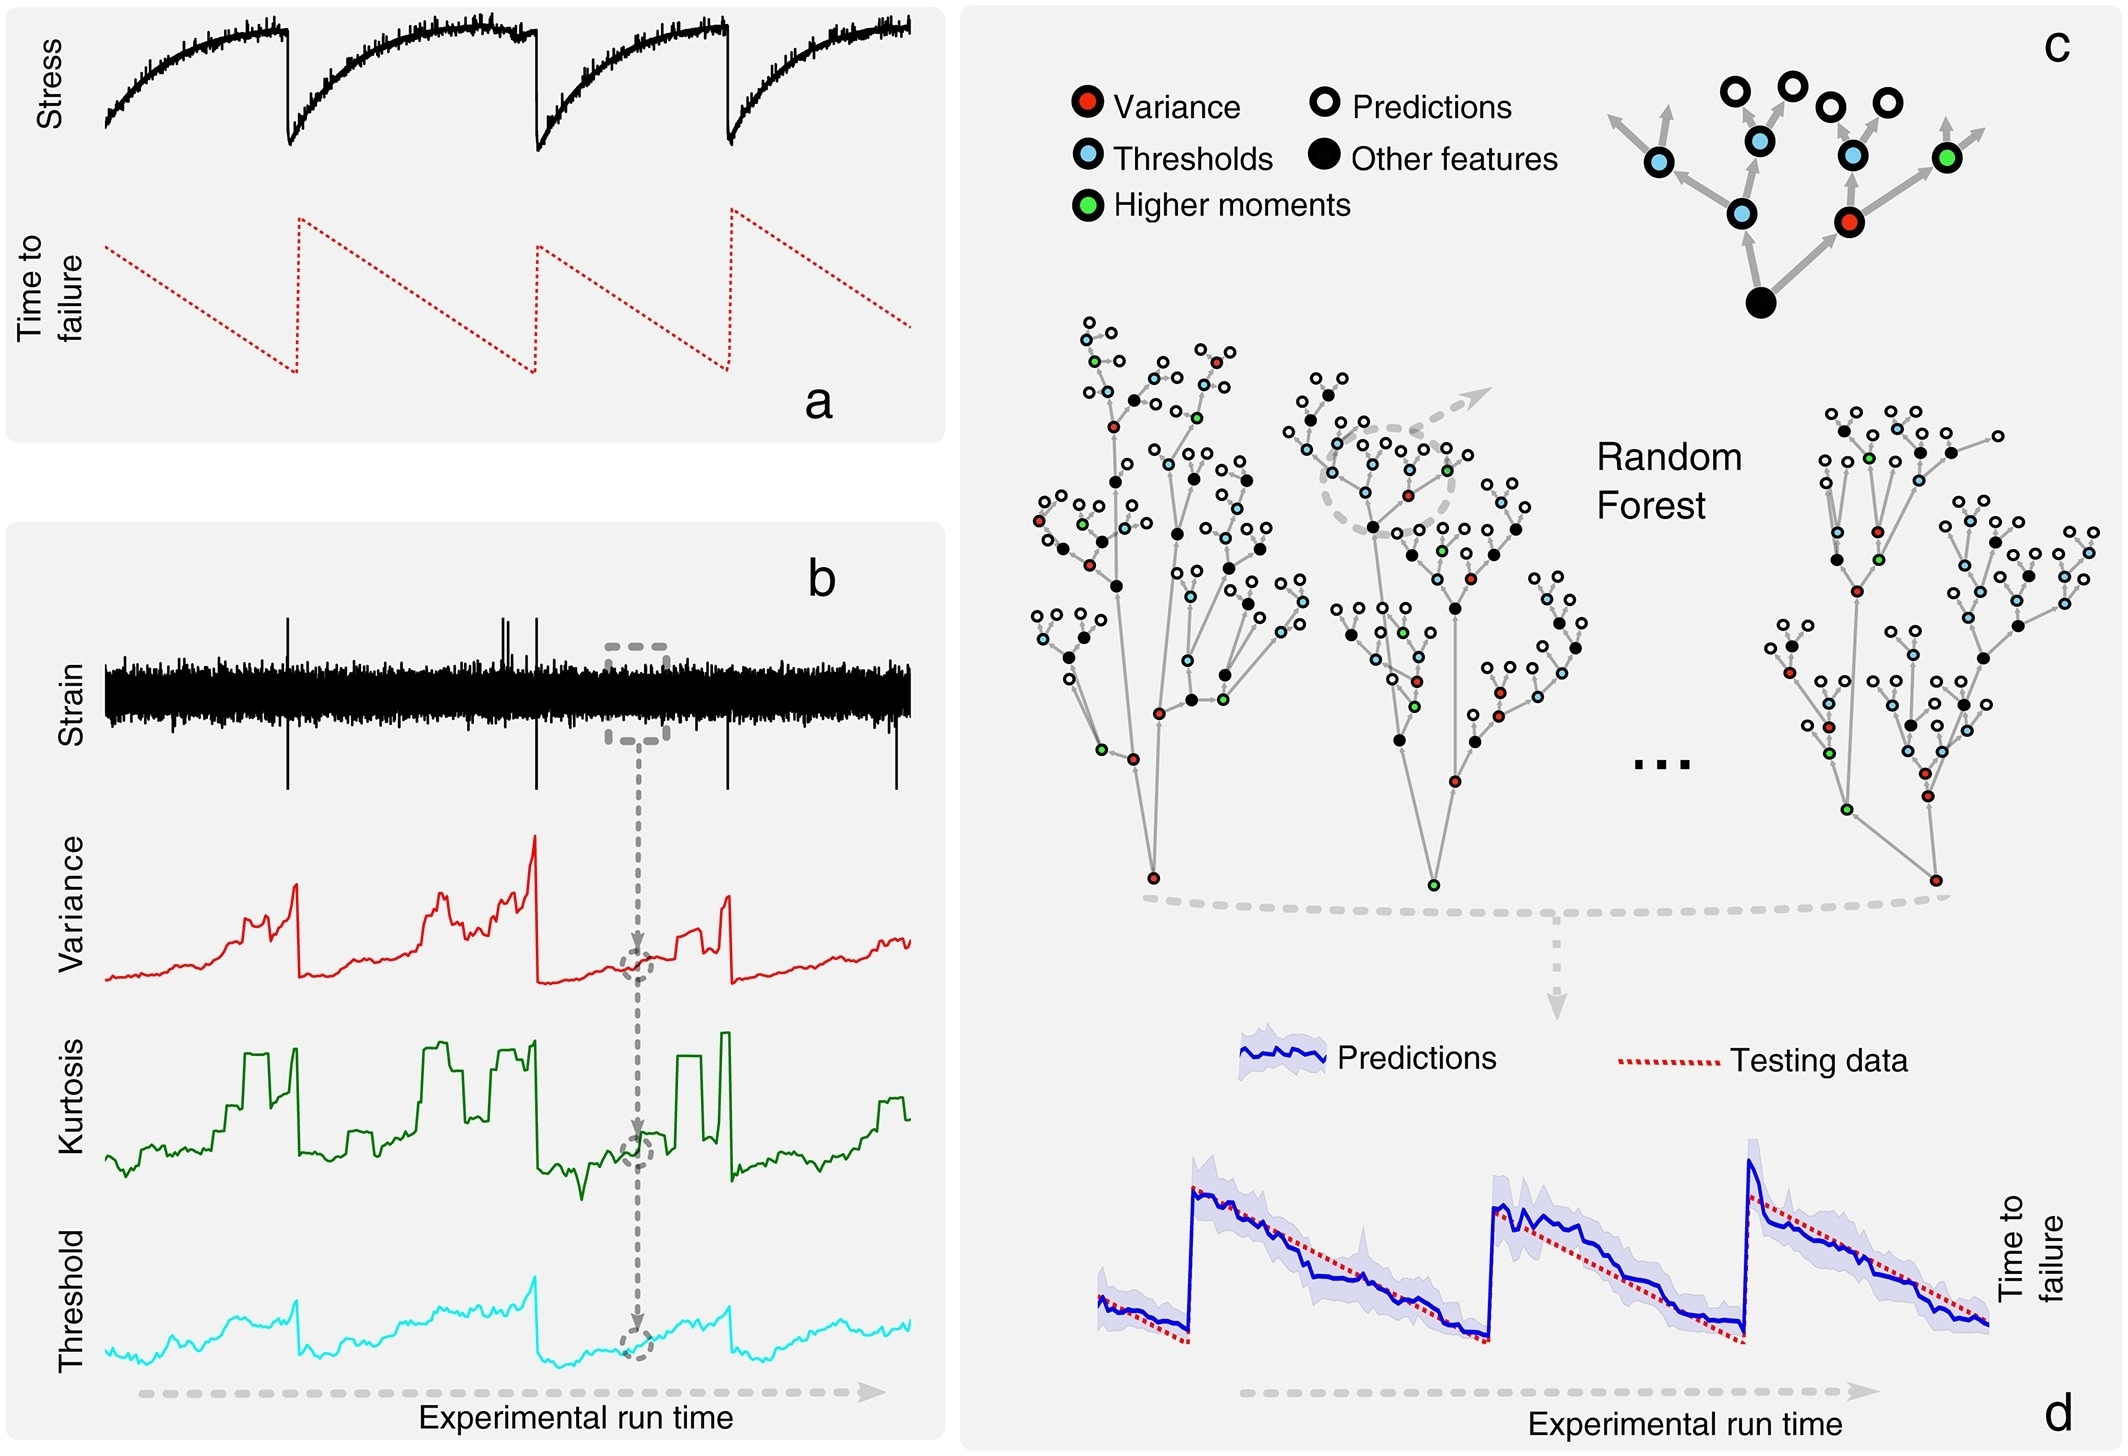
\includegraphics[width=0.7\linewidth]{pictures/grl56367-fig-0001-m.jpg}
	\caption{Random Forest (RF) approach for predicting time remaining before failure.}
	\label{fig:RF1}
\end{figure}

From each time window, a set of approximately 100 statistical features are computed, then selected recursively by usefulness, and lastly used to actually predict the time before the next earthquake. The results achieved through this study are quite accurate, even if it needs to be noted that a laboratory earthquake does not capture the physics of a complex, real-world earthquake.

\begin{figure} [h]
	\centering
	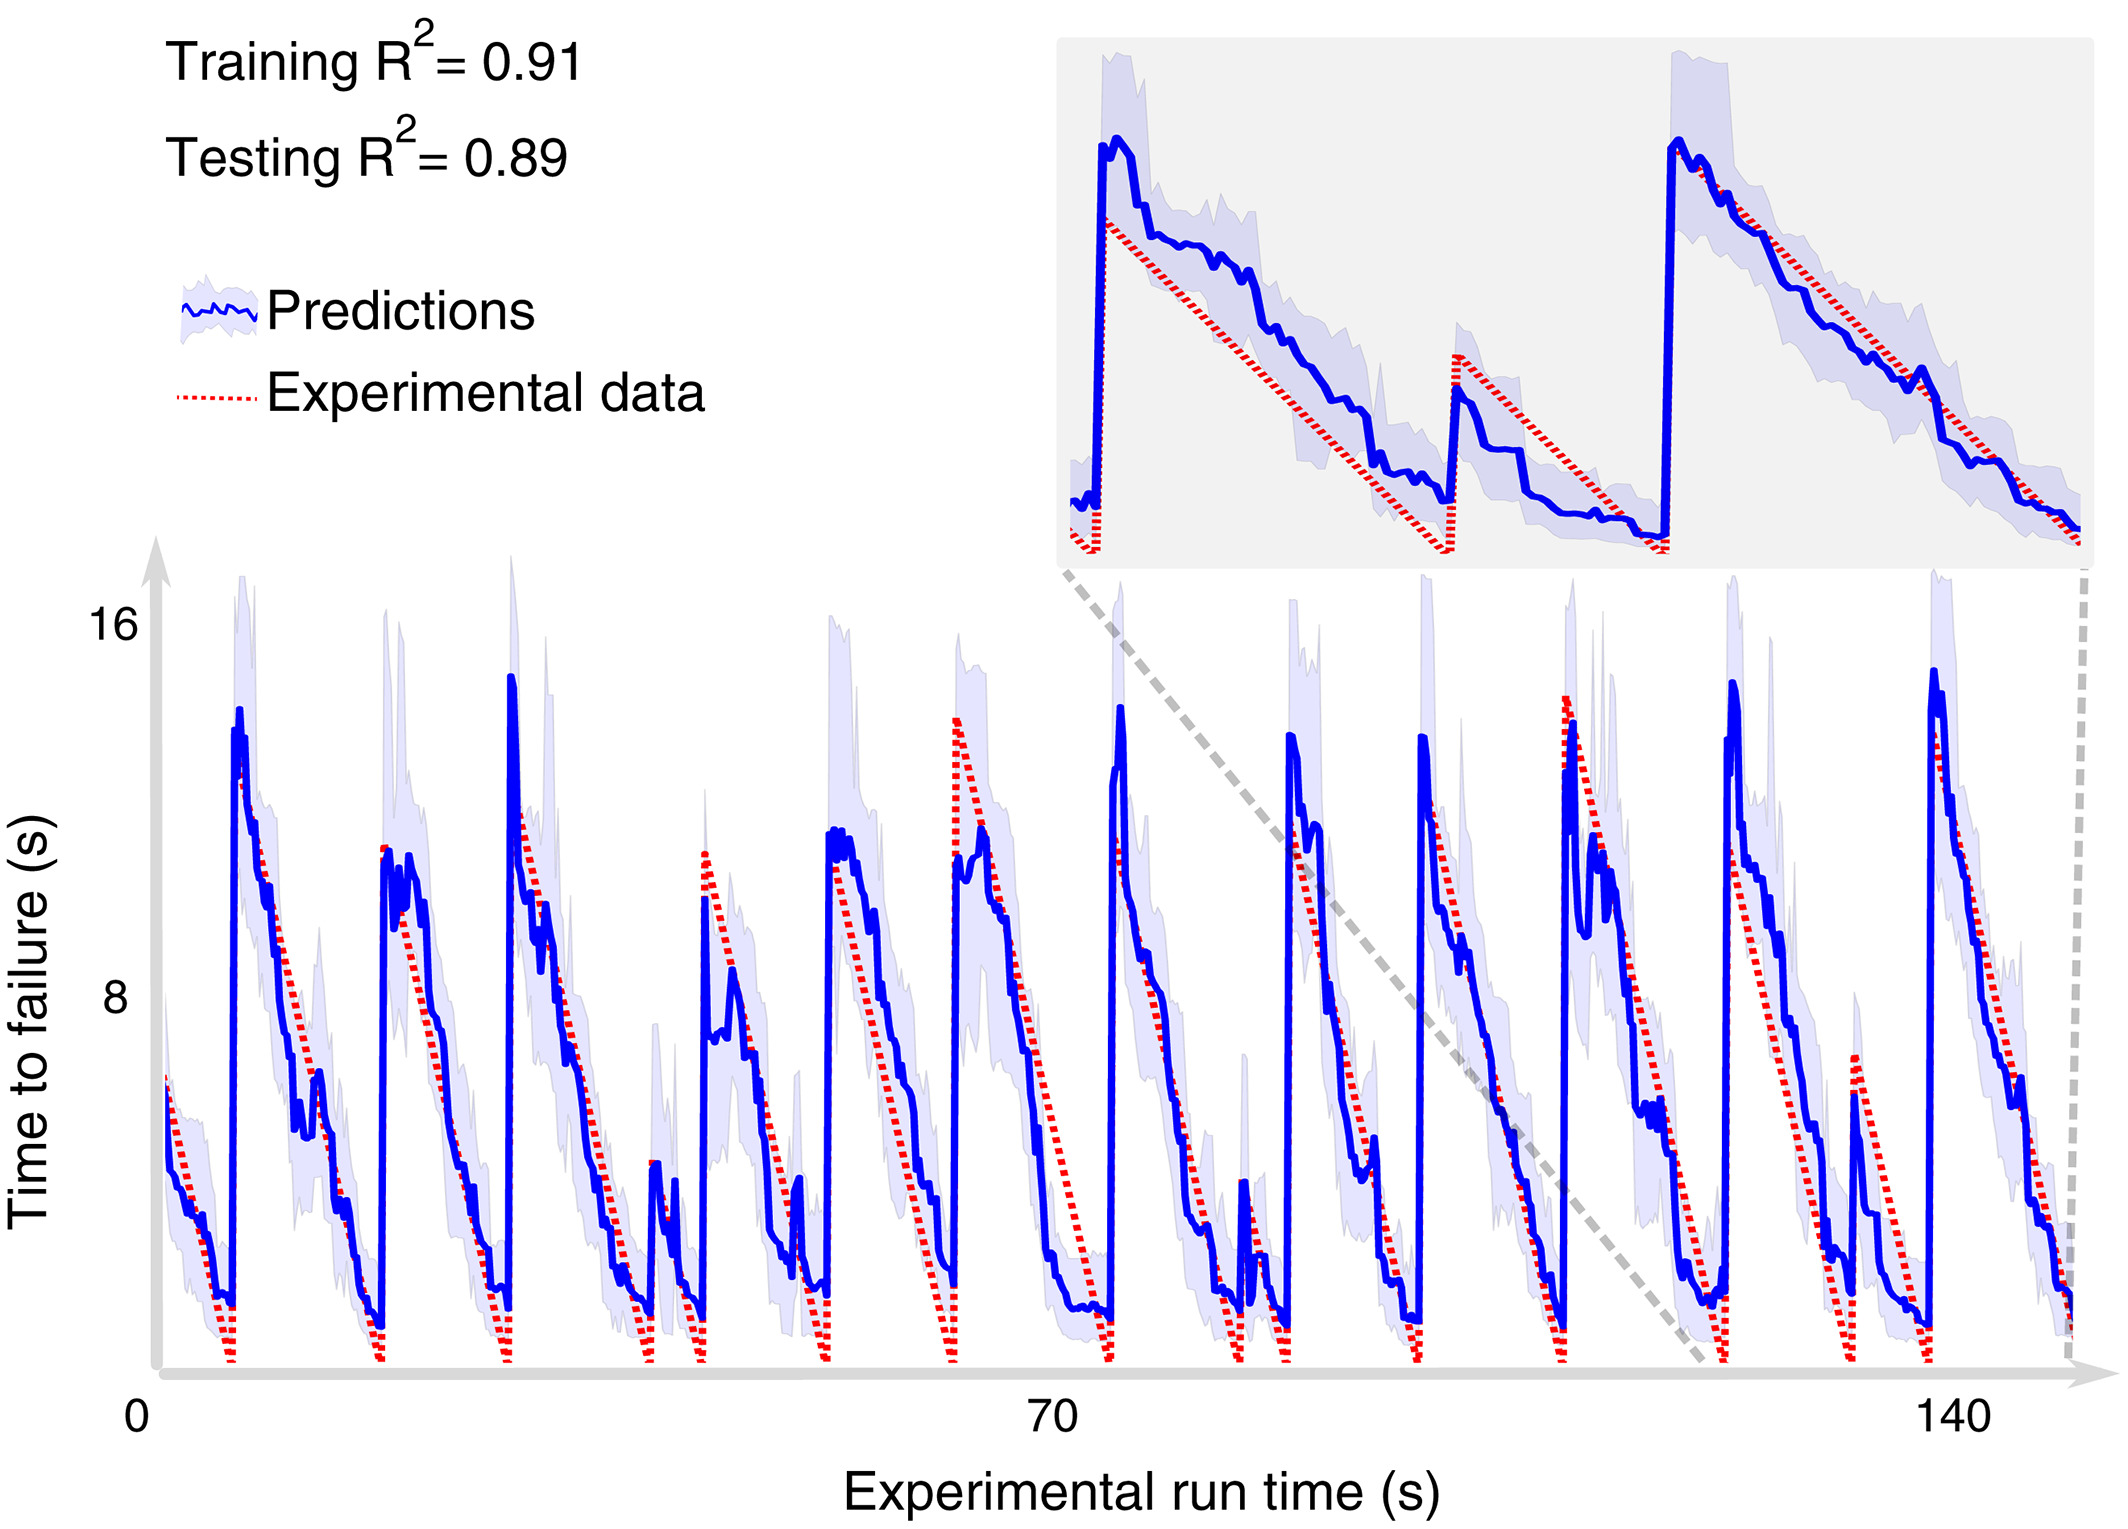
\includegraphics[width=0.7\linewidth]{pictures/grl56367-fig-0002-m.jpg}
	\caption{Time remaining before the next failure predicted by the Random Forest.}
	\label{fig:RF2}
\end{figure}

\section{Understanding the data}
With reference to the above mentioned studies, the dataset provided for the challenge contains more a-periodic occurrences of earthquake hazards, thus resembling more a real-world scenario. The data comes from a well-known experimental set-up used to study earthquake physics \cite{challenge}.

In particular, the dataset is made of two subsets:
\begin{itemize}
	\item \texttt{train.csv} - A single, continuous training segment of experimental data (with 629.145.480 entries);
	\item \texttt{test} - A folder containing many small segments (\texttt{.csv}) of test data (2.624 segments of 150.000 entries each).
\end{itemize}

\noindent Each entry of the training set has two fields:
\begin{itemize}
	\item \texttt{acoustic\textunderscore data} - the seismic signal [\texttt{int16}];
	\item \texttt{time\textunderscore to\textunderscore failure} - the time (in seconds) until the next laboratory earthquake [\texttt{float64}].
\end{itemize}

On the other hand, each segment from the test set folder is named after its \texttt{seg\textunderscore id} and only has one field, the \texttt{acoustic\textunderscore data}.
While the training set is a single, continuous, big segment of experimental data, the test set is continuous within a single segment, but the set of files cannot be considered continuous; thus, the predictions can't be assumed to follow the same pattern of the training file.

The goal of the competition is to predict a single \texttt{time\textunderscore to\textunderscore failure} for each segment, corresponding to the time between the last row of the segment and the next laboratory earthquake.

\bigbreak

A first approach to better understand what the data represents is to plot it (or a part of it, given the prohibitive size of the training set). In picture \ref{fig:plot1} we can see 1\% of the training data (obtained simply by sampling every 100 entries) \cite{kernelpreda}.

\begin{figure} [h]
	\centering
	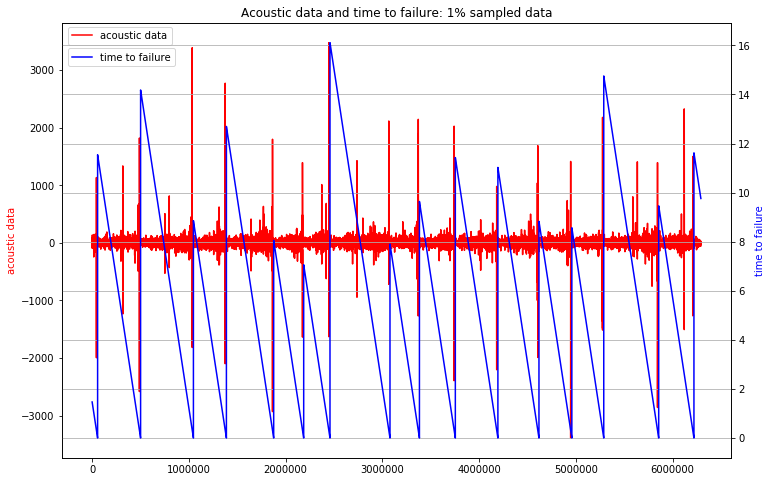
\includegraphics[width=0.7\linewidth]{pictures/plot1.png}
	\caption{Plot of 1\% sampling of the training data}
	\label{fig:plot1}
\end{figure}

The following (\ref{fig:plot2}) is instead the representation of the first 1\% entries of the training dataset: even at a first glance we are able to note that the failure ("\textit{labquake}") occurs after some medium oscillations, a very large one and some other minor ones. 

\begin{figure} [h]
	\centering
	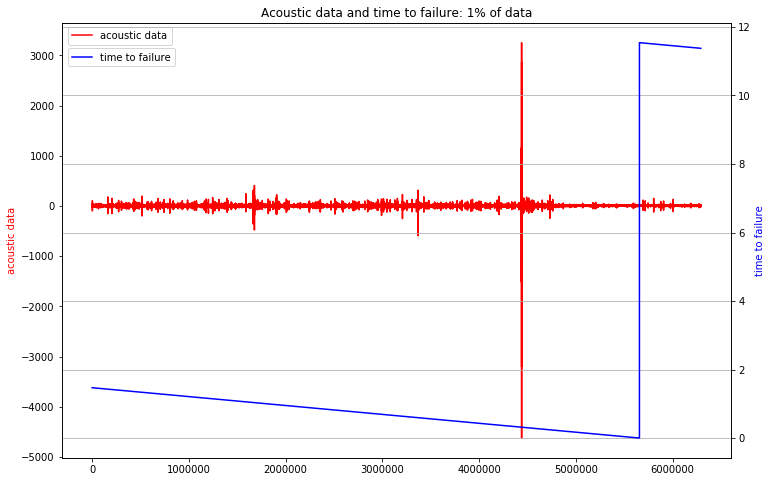
\includegraphics[width=0.7\linewidth]{pictures/plot2.png}
	\caption{Plot of the first 1\% of the training data}
	\label{fig:plot2}
\end{figure}

Before going into further details and taking a first step towards building the model from the training data, it's worth to also take a look at the structure of the test data. In picture \ref{fig:plot3} are represented four of the segments from the test folder \cite{kernelallunia}.

\begin{figure} [h]
	\centering
	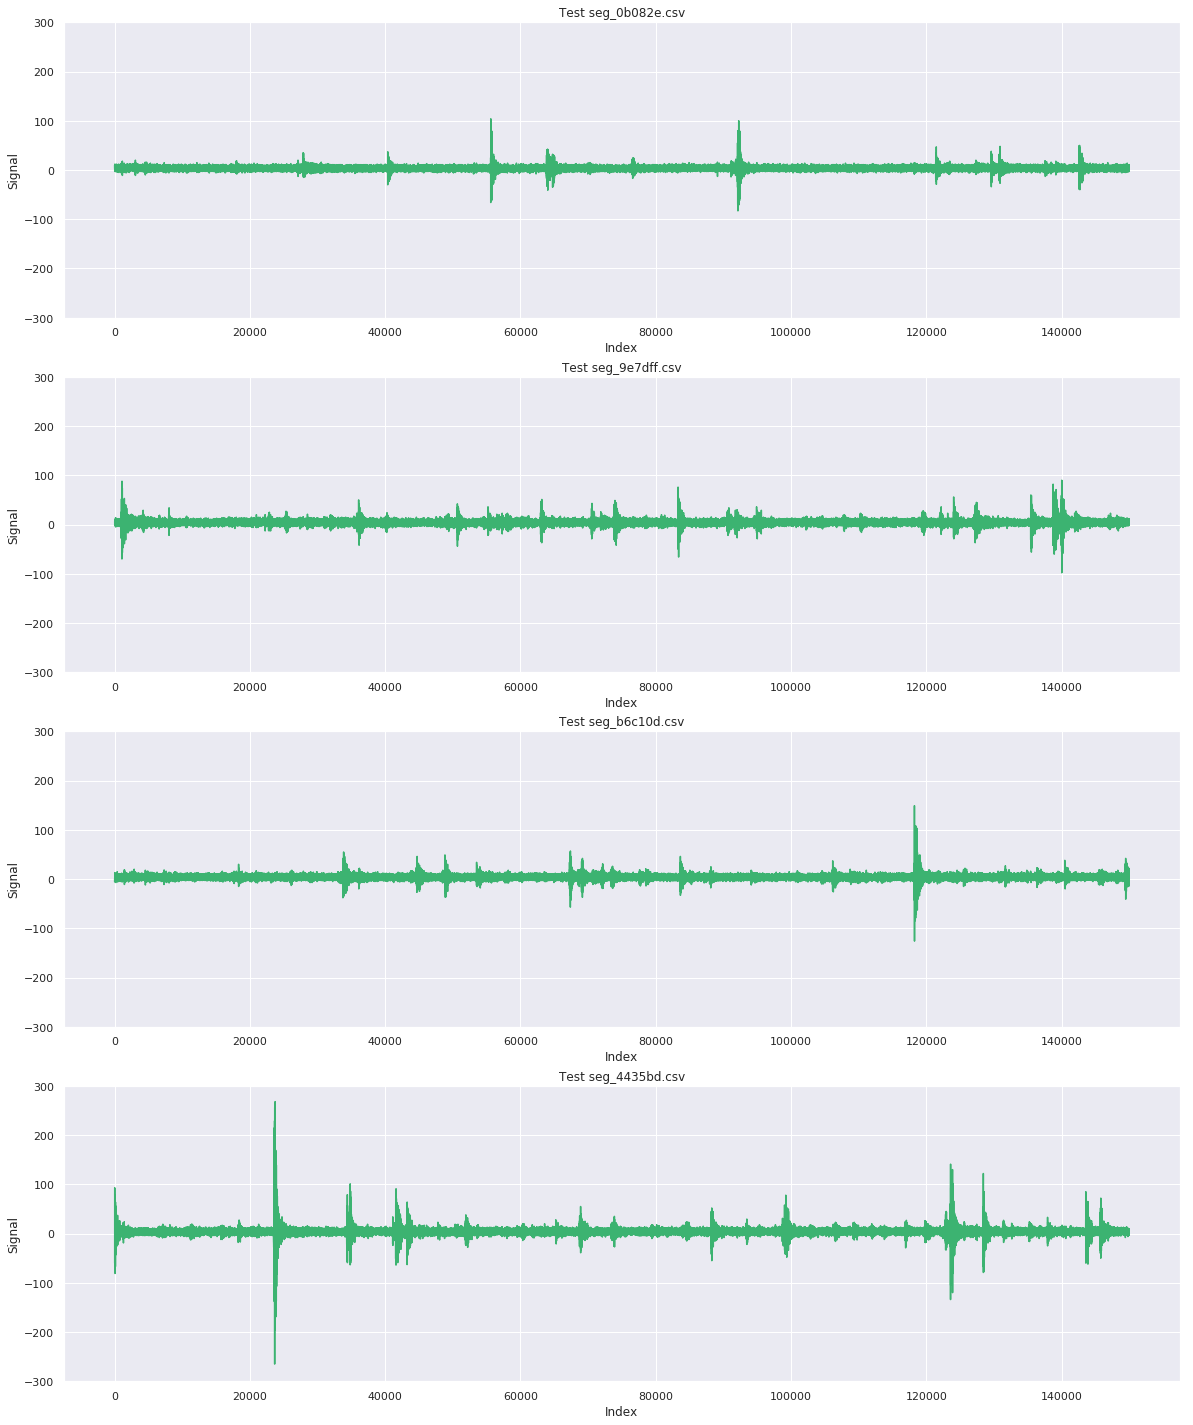
\includegraphics[width=0.7\linewidth]{pictures/plot3.png}
	\caption{Plot of four segments of the test data}
	\label{fig:plot3}
\end{figure}

\bigbreak

Overall, what we can take away from this first dive into the datasets is:
\begin{itemize}
	\item that the task of this Data Mining challenge will be in the regression spectrum, since the output falls in a continuous range rather than a set of discrete classes;
	\item that the dimension of the segments is not that big if compared to the very rare occurrences of laboratory earthquakes;
	\item that these failure events will appear very much like outliers, given the scarcity of representation and the intensity of the acoustic signal when compared to the other values.
\end{itemize}

As others participants to the challenge have noticed, it may be also relevant to note that the test set doesn't contain \textit{any} earthquake: thus, it may be worth considering not including the few failure occurrences that can be found in the training set, to avoid the model trying to match the data to these much higher peaks when fed with the test set.